\documentclass[report]{subfiles}

\begin{document}
\label{sec:implementation}

The following section will describe how the algorithms were implemented and what settings where used for each of them. It will contain no results, as they can be found in the section \ref{sec:result} \nameref{sec:result}

\subsection{Problem Setup}
\label{sec:impProblemSetup}
There are two stated problems:
\begin{itemize}
\item \textbf{Easy Problem}: The easy problem is stated as a balanced 10-fold cross validation. The data is split into 10 equal sizes, where each digit of each person is represented by the same amount. so for 3 persons with 200 of each digit and 10 different digits, each fold would include 20 of each digit of each person.
  This problem is expected to yield a better result than the hard problem, since it knows a lot about every persons method of writing a digit, before predicting the last 10 \%.  
\item \textbf{Hard Problem}: The hard problem uses cross validation as well. The difference being that each fold represent a person. For a data set of 3 persons with 200 of each digit and 10 different digits, in that case 3 folds would be created where each fold would represent just one person with all his digits.
  Opposite the easy problem, this is expected to yield a worse performance, because the training set have no previous knowledge about the person used in test. 
\end{itemize}

Both data uses digit data from 20 persons, which each has written 400 of the same digits for the digits zero to nine.

\subsubsection{Loading Images}
\label{sec:imploadingImages}
Loading of images was done using a slightly modified version of the provided algorithm for loading images.

The image loader simply loads the image and transform it into Gray-scale from RGB.
An additional flag for smoothing was added to allow smoothing of the image as seen of figure \ref{fig:loading}

\begin{figure}[H]
  \centering
  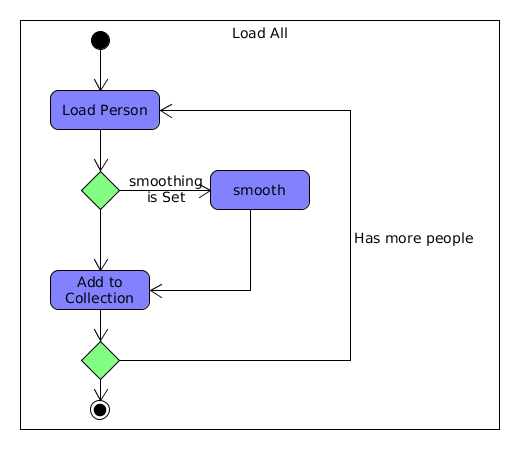
\includegraphics[width=0.4\textwidth]{UML/load}
  \caption{Shows the Activity Diagram for loading images}
  \label{fig:loading}
\end{figure}

\subsubsection{KMeans}
\label{sec:impKMeans}
KMeans can be applied in a lot of different ways.
Just to get an idea:
\begin{enumerate}
\item Perform KMeans on all digits, and based on the original class of the digit, make a vote for which digit class a cluster belong to. Say a cluster contain {1,4,4} the cluster would belong to the digit class ``4''.
\item Perform KMeans on all digits of a person. follow the same approach as above using votes to map clusters to digit class.
\item Perform KMeans on all digits of the same class.
\item Perform KMeans on all digits of the same class on each person individually
\end{enumerate}

The approach chosen has been the 4th, also shown in figure \ref{fig:kmeans}

\begin{figure}[H]
  \centering
  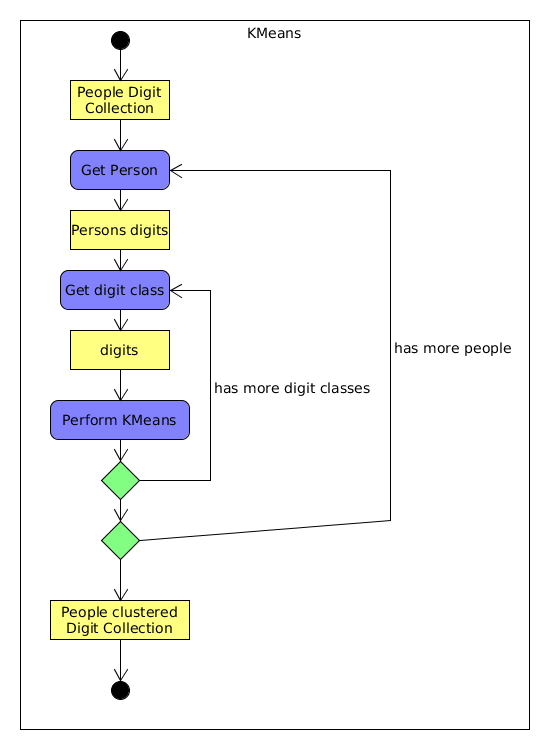
\includegraphics[width=0.6\textwidth]{UML/kmeans}
  \caption{Activity Diagram showing the use of KMeans}
  \label{fig:kmeans}
\end{figure}

\subsubsection{PCA}
\label{sec:impPCA}
The principle component analysis has been straight forward to implement.

The image data was fed to the PCA algorithm, and a percentage of the variance was extracted as amounts of principle components. Figure \ref{fig:pca} shows the flow used.

\begin{figure}[H]
  \centering
  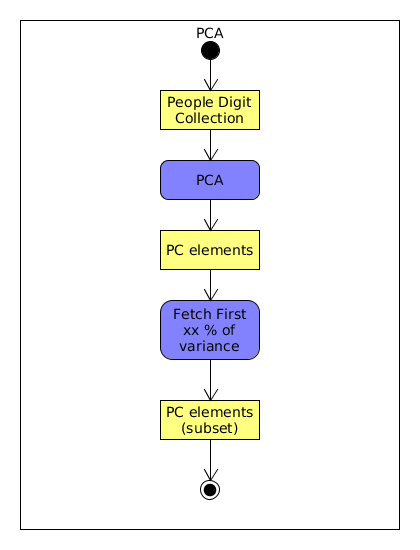
\includegraphics[width=0.5\textwidth]{UML/PCA}
  \caption{Flow for extracting PC's from the PCA to reduce less variant dimensions}
  \label{fig:pca}
\end{figure}

\subsection{KNN}
\label{sec:impKNN}

The KNN classification was done with the standard package in R, and using the pre-processing techniques Gaussian Smoothing and PCA.\\
K-Means were also tested, but the time it took to compute it was too significant and the results gave a lot lower success, both with and without the PCA. It was therefore decided not to use the k-means with KNN.

\subsubsection{Easy problem}
The easy problem was used to analyze which parameters gave the best result, because of this there are a lot of information in the resulting image.\\
The following parameters were used:
\begin{itemize}
  \item Smoothing: The default kernel were used with sigma of 0.5, 1 and 2.
  \item PCA: The variance parameters were 90\%, 95\% and 99\%.
  \item K-value: The KNN were run with the k-value of 1, 5, 10, 20 and 50.
\end{itemize}
Cross validation with a 90/10 split were performed at each preprocessing setting and at each k-value. The split was done where it takes out every tenth digit and use for testing, and then a new start index were chosen for each of the ten runs.
The results can be seen in section~\ref{sec:resultKNN} \nameref{sec:resultKNN} at figure~\ref{fig:knnEasyProblem}

\subsubsection{Hard problem}
The hard problem was calculated using the best results from the easy problem.
\begin{itemize}
  \item Smoothing: The smoothing with sigma = 1.
  \item PCA: The variance which gave the best was 99\%.
  \item K-value: The best k-value was with k = 1.
\end{itemize}
It uses the exact same way, where it only does the split different to have a whole person as test instead of data from the entire dataset.
The results can be seen in section~\ref{sec:resultKNN} \nameref{sec:resultKNN} at figure~\ref{fig:knnHardProblem}

\subsection{Random Forest}
\label{sec:impRandomForest}
Random forest has been used with all of the three pre-processing methods stated in \ref{sec:theory} \nameref{sec:theory}.

\subsubsection{Easy Problem}
\label{sec:implRF:easyProblem}

The easy problem had two flows of calculation. The two flows both have data reduction methods being KMeans versus PCA.

\begin{description}
\item[Flow 1] Using KMeans to reduce the amount of digit observations(no smoothing).
\item[Flow 2] Using PCA to reduce the amount of digit dimensions. Additionally using smoothing to reduce noise.
\end{description}

The Following Parameters was explored for the different approached:
\begin{itemize}
\item Clusters: The cluster parameters was the amount of clusters for each digit class of each person. The parameters being {10, 20, 40, 80}
\item PCA: The parameters being the amount of variance covered by principle components. the parameters being {90\%, 95\%, 99\%}
\item Smoothing: being the sigma value applied to the Gaussian kernel. The parameters being {0.5, 1, 2}
\item Number of Trees: Being the number of trees generated by the random forest algorithm. The parameters being {50, 125, 250}
\end{itemize}

\subsubsection{Hard Problem}
\label{sec:implRF:hardProblem}
The Hard problem was calculated using in two aproaches.

The first approach was:
\begin{enumerate}
\item Load Images with a smoothing parameter of sigma 1
\item Apply Kmeans with 20 clusters for each digit of each person, leaving 200 digits per person for training
\item Run Random Forest with 250 Trees
\end{enumerate}

*For testing in the Random Forest, the original digits was used, and not of the ``KMeans'' values, but the training was made from the KMeans result.  

The second Approach was:
\begin{enumerate}
\item Load Images with a smoothing parameter of sigma 1
\item Apply PCA and extract PC's covering 95 \% of the variance. 
\item Run Random Forest with 250 Trees.
\end{enumerate}

\end{document}